\section{Оптимизация с адаптивным контролем плотности 3D Гауссиан}
\label{sec:opt-dens}

Основой нашего подхода является шаг оптимизации, который создает плотный набор 3D Гауссиан, точно представляющих сцену для синтеза произвольных видов.
В дополнение к позициям $p$, $\alpha$ и ковариации $\Sigma$, мы также оптимизируем коэффициенты SH, представляющие цвет $c$ каждой Гауссианы, чтобы правильно захватывать зависимый от вида внешний вид сцены. 
Оптимизация этих параметров чередуется с шагами, контролирующими плотность Гауссиан для лучшего представления сцены.

\subsection{Оптимизация}

Оптимизация основана на последовательных итерациях рендеринга и сравнения полученного изображения с обучающими видами из захваченного набора данных. Неизбежно, геометрия может быть неправильно размещена из-за неоднозначностей проекции 3D в 2D. Таким образом, наша оптимизация должна уметь \emph{создавать} геометрию, а также \emph{уничтожать} или \emph{перемещать} геометрию, если она была неправильно расположена. Качество параметров ковариаций 3D Гауссиан критично для компактности представления, поскольку большие однородные области могут быть захвачены небольшим числом крупных анизотропных Гауссиан.

Мы используем методы стохастического градиентного спуска для оптимизации, полностью используя стандартные GPU-ускоренные фреймворки\TODO{ДОБАВИТЬ ссылку на pytorch}, и возможность добавлять пользовательские CUDA-ядра для некоторых операций, следуя современным рекомендациям~\cite{plenoxels,dvgo-cvpr2022}. В частности, наш быстрый растеризатор (см. Раздел~\ref{sec:tile-raster}) критичен для эффективности нашей оптимизации, поскольку это основное вычислительное узкое место оптимизации.

Мы используем сигмоидальную функцию активации для $\alpha$, чтобы ограничить её диапазоном $[0-1)$ и получить гладкие градиенты, и экспоненциальную функцию активации для масштаба ковариации по аналогичным причинам.

Мы оцениваем начальную ковариационную матрицу как изотропную Гауссиану с осями, равными среднему расстоянию до ближайших трех точек. 
Мы используем стандартную технику экспоненциального затухания, аналогичную Plenoxels~\cite{plenoxels}, но только для позиций. Функция потерь представляет собой комбинацию $\mathcal{L}_1$ и терма D-SSIM:

\begin{equation}
    \mathcal{L} = (1 - \lambda) \mathcal{L}_1 + \lambda \mathcal{L_{\textrm{D-SSIM}}}
\end{equation}

Мы используем $\lambda~=~0.2$ во всех наших тестах.
Подробнее о расписании обучения и других элементах представлено в Разделе~\ref{sec:impl}.

\subsection{Адаптивный контроль Гауссиан}

Мы начинаем с начального набора разреженных точек из SfM, а затем применяем наш метод для адаптивного контроля \REMOVAL{плотности \Dg~}\CORRECTION{количества 3D Гауссиан и их плотности на единицу объема}{числа Гауссиан и их плотности на единицу объема}\footnote{Плотность \CORRECTION{\Dg~}{Гауссиан} не следует путать, конечно же, с плотностью $\sigma$ в литературе NeRF.}, что позволяет нам перейти от начального разреженного набора Гауссиан к более плотному набору, который лучше представляет \CORRECTION{экран}{сцену} и имеет правильные параметры. 
После прогрева оптимизации (см. Раздел~\ref{sec:impl}), мы уплотняем каждые 100 итераций и удаляем любые Гауссианы, которые практически прозрачны, то есть с $\alpha$ меньше порога $\epsilon_{\alpha}$.

Наш адаптивный контроль \CORRECTION{плотности \Dg~}{Гауссиан} должен заполнять пустые области. Он фокусируется на областях с отсутствующими геометрическими особенностями («недостаточная реконструкция»), но также и в областях, где Гауссианы покрывают большие области сцены (что часто соответствует «чрезмерной реконструкции»).
\TODO{МОЖЕТ БЫТЬ ДОБАВИТЬ РИСУНОК (GK)}
Мы наблюдаем, что у обоих случаев есть \emph{большие} градиенты положения в пространстве видов.
Интуитивно это объясняется тем, что они соответствуют областям, которые еще не хорошо реконструированы, и оптимизация пытается переместить Гауссианы для исправления этого.

Поскольку оба случая являются хорошими кандидатами для уплотнения, \CORRECTION{следовательно}{} мы
уплотняем Гауссианы со средней величиной градиента положения в пространстве видов выше порога~$\tau_{\textrm{pos}}$, который мы установили равным $0.0002$ в наших тестах.

Далее мы представляем подробности этого процесса, проиллюстрированные на Рис.~\ref{fig:density_control}.

\begin{figure}[!h]
    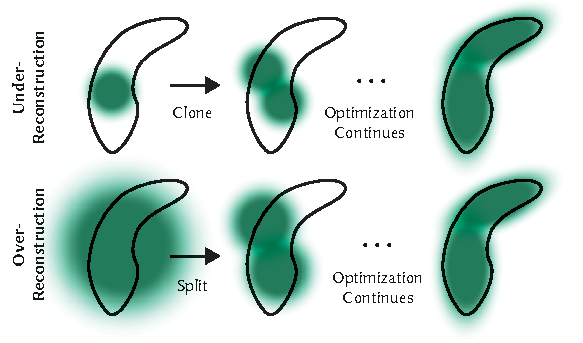
\includegraphics[width=\linewidth]{figures/density_control/density_control_01.pdf}
    \caption{
        \label{fig:density_control}
        Наша адаптивная схема уплотнения Гауссиан.
        \emph{Верхний ряд (недостаточная реконструкция)}: Когда мелкомасштабная геометрия (черный контур) недостаточно покрыта, мы клонируем соответствующую Гауссиану.
        \emph{Нижний ряд (чрезмерная реконструкция)}: Если мелкомасштабная геометрия представлена одним большим сплатом, мы разделяем его на два.
    }
\end{figure}

Для маленьких Гауссиан в недостаточно реконструированных регионах нам нужно покрыть новую геометрию, которая должна быть создана.
Для этого предпочтительно клонировать Гауссианы, просто создавая копию того же размера и перемещая её в направлении градиента положения.

С другой стороны, крупные Гауссианы в регионах с высокой дисперсией должны быть разделены на меньшие Гауссианы. Мы заменяем такие Гауссианы\REMOVAL{таким образом удаляем такие Гауссианы и вводим} двумя новыми\REMOVAL{Гауссианами}, и делим их масштаб на множитель $\phi~=~1.6$, который мы определили экспериментально.
Мы также инициализируем их положение, используя исходную 3D Гауссиану как PDF для выборки.

В первом случае мы обнаруживаем и лечим необходимость \CORRECTION{увеличения плотности \Dg}{увеличения как общего объема системы, так и количества Гауссиан}, тогда как во втором случае мы сохраняем \CORRECTION{общую плотность \Dg~ системы.}{общий объем, но увеличиваем количество Гауссиан.}
\CORRECTION{Учитывая, что наша задача не является строго выпуклой, оптимизация иногда может застрять в локальных минимумах, что может привести к необоснованному увеличению плотности Гауссиан.}{Подобно другим объемным представлениям, наша оптимизация может застрять с "плавающими" объектами близко к входным камерам; в нашем случае это может привести к необоснованному увеличению плотности Гауссиан.}
Эффективный способ умерить увеличение числа Гауссиан \CORRECTION{и справиться с плавающими объектами} — установить значение $\alpha$ близкое к нулю каждые $N=3000$ итераций. Затем оптимизация увеличивает $\alpha$ для Гауссиан, где это необходимо, позволяя нашему подходу удаления исключать Гауссианы с $\alpha$ меньше $\epsilon_{\alpha}$, как описано выше. \CORRECTION{Мы также}{Гауссианы могут сжиматься или расширяться и значительно пересекаться с другими, но мы периодически} удаляем \CORRECTION{}{Гауссианы, которые являются} очень большими \CORRECTION{Гауссианы} в мировом пространстве и \CORRECTION{Гауссианы}{те, что} имеют большой след в пространстве видов. Эта стратегия обеспечивает хорошее общее управление общим числом Гауссиан. \ADDITION{Гауссианы в нашей модели остаются примитивами в евклидовом пространстве в любое время; в отличие от других методов~\cite{barron2022mipnerf360,plenoxels}, нам не требуются стратегии уплотнения пространства, деформации или проекции для дальних или больших Гауссиан.}